\documentclass[a4paper,8pt,twocolumn]{article}
\usepackage[utf8]{inputenc}%codification of the document
\usepackage{geometry}
\geometry{hmargin=1cm, vmargin=1cm}

\usepackage{graphicx}
\graphicspath{ {./images/} }

\title{RAPPORT: TRANSPORT OPTIMAL}
\author{ANDRIAMAHERISOA Liantsoa}
\date{Juin 2020}

%Here begins the body of the document
\begin{document}
\begin{titlepage}
\maketitle
\end{titlepage}
\section{Introductions}
    Le principe du chemin le plus court guide la plupart des décisions dans les domaines de la vie et des sciences: lorsqu’un produit, une personne ou un seul élément d’information est disponible à un point donné et doit être accessible à envoyer à un point cible. Il convient de privilégier le moins d’effort possible.  La théorie du transport optimal (TO) généralise cette intuition dans le cas où, au lieu de déplacer un seul élément à la fois, on se préoccupe du problème de déplacement simultanément de plusieurs éléments (ou une distribution continue de ceux-ci) d’un espace à un autre. \newline Introduite au 18ème siècle, ce n’est que récemment que cette théorie constitue un terrain fertile pour les chercheurs en informatique, en imagerie et plus généralement en sciences des données car cette théorie fournissait des outils très puissant pour étudier les distributions dans un contexte différent et plus abstrait, celui de comparer les distributions, facilement disponibles sous la forme d’un sac de caractéristiques ou d’informations. Maintenant que le TO s’est progressivement imposé comme un outil informatique, centré sur les applications à la science des données, notamment, l’imagerie et l’apprentissage automatique.
\section{Fondements Théoriques}
    Ici, nous allons introduire les notions relatives d’appariements et de couplage optimaux entre vecteurs de probabilité (a, b), généralisant progressivement ce calcul pour un transporter des mesures discrètes  ($\alpha, \beta$), pour couvrir enfin le cadre général des mesures arbitraires.
\subsection{Histogrammes et Mesures}
    On utilise de manière interchangeable les termes histogramme et vecteur de probabilité pour tout élément a $\[\in\sum_{n}$  qui appartient au simplexe de probabilité. \newline
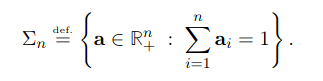
\includegraphics[width=0.3\textwidth]{histogram an measure}\newline
    Pour des mesures discrètes avec des poids a et les emplacements $x_1$, … , $x_n$ $\in$ X.
    Noté:\newline
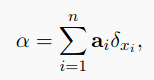
\includegraphics[width=0.15\textwidth]{mesure discret.png}\newline
    où $\sigma$x est le Dirac à la position x, intuitivement une unité de masse est concentrée à l’infini au position x.
    Cette mesure décrit une mesure de probabilité si, en plus,  a $\[\in\sum_{n}$ et plus généralement une mesure positive si tous les éléments du vecteur sont non négatifs.\newline

    Pour les mesures en générales: discrètes ou continues. On s’appuie sur l’ensemble des mesure de Randon M(X) sur l’espace X. X doit être accompagné d’une distance d, car on ne peut accéder à une mesure qu’en l’intégrant contre les fonctions continues, notés f$\in$C(X):\newline
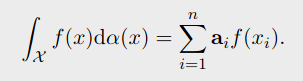
\includegraphics[width=0.28\textwidth]{mesure general}\newline
\subsection{Affectation et problème de Monge}
    Dans ce cas, on va avoir une matrice de coût\newline	
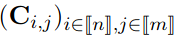
\includegraphics[width=0.2\textwidth]{f5.png}\newline
    En supposant n = m, le problème d’affectation optimal cherche une bijection $\sigma$ dans l’ensemble Perm(n) des permutations d’éléments. On cherche alors à faire:\newline
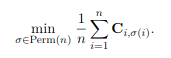
\includegraphics[width=0.2\textwidth]{monge.png}\newline
    Une méthode naïve est d’évaluer cette fonction coût en  utilisant toutes les permutations dans l’ensemble Perm(n). Cependant, cet ensemble a une taille n! Qui est énorme même pour des petits n. On va devoir utiliser des algorithmes efficaces pour optimiser le calcul.
    Le problème d’affection optimale peut avoir plusieurs solutions optimales, comme par exemple dans le cas de deux éléments identiques, on peut avoir deux affectations possibles qui sont tout les deux optimales.\newline
    
    Dans le cas de mesures discrètes, le problème Monge cherche une carte qui associe à chaque point $\[x_i\]$ un seul point  $\[y_j\]$ et qui va pousser la masse de $\alpha$ vers la masse de $\beta$. Une telle carte T doit vérifier:\newline
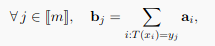
\includegraphics[width=0.25\textwidth]{monge 2.png}\newline

    Dans le cas de mesures arbitraires ($\alpha,\beta$), supposant deux espaces (X, Y) peuvent être liés par une carte 
    T:X $\rightarrow$ Y qui minimise:\newline
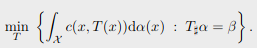
\includegraphics[width=0.3\textwidth]{monge 3.png}\newline
    La contrainte $\[$T_\mp_\alpha\] = $\beta$  veut dire que T pousse en avant la masse de $\alpha$ vers la masse de $\beta$, en utilisant la méthode de «push-forward».
    La nature combinatoire du problème dans le cas discret et la complexité de la contrainte  $\[$T_\mp_\alpha\]$ qui est convexe font que le problème de Monge est très difficile.
    
\subsection{La formulation relaxée de Kantorovich}

    Puisque le problème de Monge est trop ardu, il faut nous résigner à en résoudre un plus simple. C’est la stratégie proposée par Kantorovich. 
    Plutôt que d’exiger que l’élément x d’une distribution $\alpha$ soit transporté de manière déterministe vers un point T(x) dans la distribution cible $\beta$, Kantorovich propose d’autoriser la répartition des éléments sur différents points dans la cible. 
    Un plan de transport $\gamma$ entre deux distributions discrètes $\alpha$ et $\beta$. La masse d’un point dans $\alpha$ peut être répartie sur plusieurs points dans $\beta$. 
    $\gamma$(x,y) est une distribution de probabilités jointe qui indique la proportion d’élément au voisinage de x dans $\alpha$ que l’on va transporter au voisinage de y dans $\beta$. Pour que ce plan de transport soit compatible avec  $\alpha$ et $\beta$ il faut exiger les contraintes de marginalité . Cette flexibilité est alors codée en utilisant, à la place  d’une permutation $\sigma$ ou une carte T, une matrice de couplage ${P}$\in\[${R}({n}$\times$ {m})_+\]$ , où $P_i,j}$ décrit la quantité de masse circulant de i vers j, ou de la masse trouvée en $x_i$ vers $y_j$. Les couplages admissibles admettent une caractérisation beaucoup plus simple que les cartes Monge, 
    où, on utilise la matrice vectorielle suivante: \newline
    
    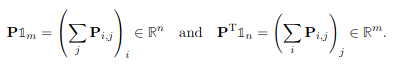
\includegraphics[width=0.4\textwidth]{images/kantorovich3.png}\newline
    L’ensemble des matrices U(a,b) est borné et défini par n+m contraintes d’égalité, et est donc un polytope convexe (la coque convexe d’un ensemble fini de matrices). De plus, alors que la formulation de Monge était intrinsèquement asymétrique, la formulation détendue de 
    Kantorovich est toujours symétrique, dans le sens où un couplage P est dans U(a,b) si et seulement si $P^T$. est dans U(b,a), d’où:}\newline
    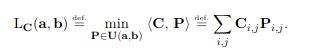
\includegraphics[width=0.35\textwidth]{images/Kantarovich4.png}\newline
    C’est une problème linéaire, et comme c’est généralement le cas avec de telles problèmes, ses solutions optimales ne sont pas forcément uniques. \newline
    
    \textbf{Matrices de permutation comme couplages:} Pour une permutation $\sigma\in$Perm(n), on écrit P$\sigma$ pour la matrice de permutation correspondantes:\newline
    \includegraphics[width=0.35\textwidth]{images/kantorovich5.png}\newline
    Pour le cas des mesures discrètes, nous stockons dans la matrice C tous les coûts par paire entre les points dans les supports de $\alpha$, $\beta$, à savoir $C_i{,}_j$ = c($x_i$, $y_j$), pour définir:\newline
     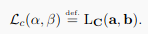
\includegraphics[width=0.25\textwidth]{images/KANTOROVICH6.png}\newline  
    
    Par conséquent, la formulation de Kantorovich du TO entre
    les mesures discrètes est la même que le problème entre leurs vecteurs de probabilité de poids a,b sauf que la matrice de coût C dépend du support de $\alpha$ et $\beta$.
    Dans le cas des mesures arbitraires, $L_c$ est étendu à des mesures arbitraires en considérant les couplages $\pi$\in$M^1_+$ (X$\times$Y) qui sont des distributions conjointes sur l’espace produit. Le cas discret est une situation particulière où l'on impose que cette mesure de produit soit de la forme $\pi$ = $\sum_i{,}_j$ P$_i{,}_j$\delta($x_i$, $y_j$). Dans le cas général, la contrainte de conservation de la masse doit être réécrite en tant que contrainte marginale sur la distribution de probabilité conjointe.\newline  
    
     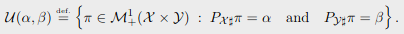
\includegraphics[width=0.45\textwidth]{images/kantorovich7.png}\newline  
     
\subsection{Propriétés métriques du TO : Wasserstein}

    Pour définir une notion de distance entre deux distributions $\alpha$ et $\beta$, on utilise la distance de p-Wasserstein entre $\alpha$ et $\beta$. Pour la fonction de coût de transport C on choisit C(x,y) = $D^p$ (x,y) où D(x,y) est une distance entre x et y et où p $\geq$ 1.\newline 

     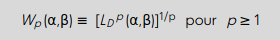
\includegraphics[width=0.29\textwidth]{images/wasserstein1.png}\newline  
     
    On doit vérifier: $W_p$ ($\alpha$, $\gamma$) $\geq$ $W^p$ ($\alpha$, $\beta$) + Wp ($\beta$, $\gamma$). \newline
    Dans certains cas spécifiques ont peut néanmoins $W^p$ explicitement: \newline
    
    - distance entre deux distributions $\alpha$ = $\delta_{x}$ et $\beta$ = $\delta_{y}$, on vérifie immédiatement que $W_p$ ($\delta_x$, $\delta_y$) = D(x,y)\newline
    
    - dans le cas p = 2, si l’on définit $\alpha^’$ et $\beta^’$ comme les versions centrées de moyennes nulles $\alpha$ et $\beta$, qu’on définit $m_\alpha$ et $m_\beta$ comme les moyennes respectives de $\alpha$ et $\beta$ alors on a la décomposition
    	$W_2\(($\alpha$,$\beta$)^2$ = $W_2\(($\alpha^'$,$\beta^'$)^2$ + $\|$$m_\alpha$ – $m_\beta$ $\|^2$.$ \newline
    	
    - dans le cas p = 2 avec deux gaussiennes $\alpha$ = N($m_\alpha$, $\sum_\alpha$) et $\beta$ = N($m_\beta$, $\sum_\beta$, on a:
	$W_2\(($\alpha$,$\beta$)^2$ = $\|$$m_\alpha$ – $m_\beta$ $\|^2 + B($\sum_\alpha$ , $\sum_\beta$) où B est une métrique entre matrices de covariances que l’on sait calculer explicitement.\newline
	
\subsection{Problème Dual}

    Le problème de Kantorovich est un problème de minimisation convexe avec contraintes et, par conséquent, il peut naturellement être associé à un problème dual, qui est un problème de maximisation concave avec contraintes.
    Le problème de Kantorovich admet:\newline
    
    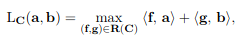
\includegraphics[width=0.35\textwidth]{images/Dual1.png}\newline 
    où, l’ensemble des variables duals est:\newline 
    
    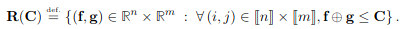
\includegraphics[width=0.5\textwidth]{images/dual2.png}\newline 
    
    appelées «potentiels de Kantorovich».
    Ce résulta est une conséquence directe du résultat plus général sur la forte dualité des programmes linéaires. 
    Déduisons notre résultat en utilisant la dualité Langrangienne. D’où: \newline 
    
    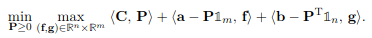
\includegraphics[width=0.47\textwidth]{images/dual3.png}\newline 
    En échangeant le min et le max, on obtient:
    
    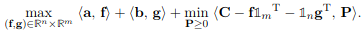
\includegraphics[width=0.47\textwidth]{images/dual4.png}\newline 
    On en conclu grâce à ce remarque: \newline 
    
    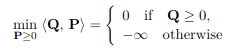
\includegraphics[width=0.3\textwidth]{images/dual5.png}\newline 
    de sorte que la contrainte se lit \newline
    
    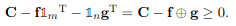
\includegraphics[width=0.3\textwidth]{images/dual6.png}\newline
    
    Ainsi, la relation d’optimalité primale-dual pour le lagrangien permet de localiser le support du plan de transport optimal. 
        
\end{document}

